\documentclass[12pt]{article}
\usepackage[margin=1in]{geometry}
\usepackage{amsmath,amsthm,amssymb}

% Ignore spaces in filenames
\usepackage[space]{grffile}

\usepackage[T1]{fontenc}
\usepackage{bigfoot} % to allow verbatim in footnote
\usepackage[numbered,framed]{matlab-prettifier}
\usepackage{filecontents}
\usepackage{graphicx}
\usepackage[normalem]{ulem}

\let\ph\mlplaceholder % shorter macro
\lstMakeShortInline"

\lstset{
  style              = Matlab-editor,
  basicstyle         = \mlttfamily,
  escapechar         = ",
  mlshowsectionrules = true,
}

\title{MAE 275 - Homework 4}
\author{John Karasinski}

\begin{document}
\maketitle

\section{Defining the System}
The longitudinal linearized aircraft equations of motion can be expressed in state space form, with state variables $\Delta u, \Delta w, \Delta q, \Delta \theta, \Delta h$, as
% \begin{equation}
% \begin{split}
% \Delta \dot{u} = &X_u \Delta u + X_w \Delta w - g\cos \theta_0 \Delta \theta + \sum\limits_{i=1}^n X_{\delta_i} \Delta \delta_i \\
% \Delta \dot{w} = &\dfrac{Z_u}{1-Z_{\dot{w}}} \Delta u +
%                   \dfrac{Z_w}{1-Z_{\dot{w}}} \Delta w +
%                   \dfrac{Z_q + u_0}{1-Z_{\dot{w}}} \Delta q -
%                   \dfrac{g\sin \theta_0}{1-Z_{\dot{w}}} \Delta \theta +
%                   \dfrac{1}{1-Z_{\dot{w}}} \sum\limits_{i=1}^n Z_{\delta_i} \Delta \delta_i \\
% \Delta \dot{q} = &\left[ M_u + \dfrac{M_{\dot{w}} Z_u}{1-Z_{\dot{w}}} \Delta u  \right] +
%                   \left[ M_w + \dfrac{M_{\dot{w}} Z_w}{1-Z_{\dot{w}}} \Delta w  \right] +
%                   \left[ M_q + \dfrac{M_{\dot{w}} (Z_q + u_0)}{1-Z_{\dot{w}}} \Delta q  \right] \\
%                  & - \left[ \dfrac{M_{\dot{w}} g\sin \theta_0}{1-Z_{\dot{w}}} \Delta \theta  \right]
%                    + \dfrac{M_{\dot{w}}}{1-Z_{\dot{w}}} \sum\limits_{i=1}^n Z_{\delta_i} \Delta \delta_i
%                    + \sum\limits_{i=1}^n M_{\delta_i} \Delta \delta_i \\
% \Delta \dot{\theta} = &\Delta q \\
% \end{split}
% \label{long}
% \end{equation}

\begin{equation*}
A =
\begin{bmatrix}
    X_u & X_w & 0 & -g \cos(\theta_0) & 0 \\
    \dfrac{Z_u}{1-Z_{\dot{w}}} & \dfrac{Z_w}{1-Z_{\dot{w}}} & \dfrac{Z_q + u_0}{1-Z_{\dot{w}}} & -\dfrac{g\sin \theta_0}{1-Z_{\dot{w}}} & 0 \\
    M_u + \dfrac{M_{\dot{w}} Z_u}{1-Z_{\dot{w}}} & M_w + \dfrac{M_{\dot{w}} Z_w}{1-Z_{\dot{w}}} & M_q + \dfrac{M_{\dot{w}} (Z_q + u_0)}{1-Z_{\dot{w}}} & -\dfrac{M_{\dot{w}} g\sin \theta_0}{1-Z_{\dot{w}}} & 0 \\
    0 & 0 & 1 & 0 & 0 \\
    0 & -1 & 0 & u_0 & 0
\end{bmatrix}
\end{equation*}

\noindent Relevant B, C, and D matrices can also be formed
\begin{equation*}
B =
\begin{bmatrix}
-X_u                                          & -X_w                                          & 0                                               & X_{\delta_e} \\
\dfrac{-Z_u}{1-Z_{\dot{w}}}                   & \dfrac{-Z_w}{1-Z_{\dot{w}}}                   & \dfrac{-Z_q}{1-Z_{\dot{w}}}                     & \dfrac{Z_{\delta_e}}{1-Z_{\dot{w}}} \\
-M_u - \dfrac{M_{\dot{w}} Z_u}{1-Z_{\dot{w}}} & -M_w - \dfrac{M_{\dot{w}} Z_w}{1-Z_{\dot{w}}} & -M_q -\dfrac{M_{\dot{w}} (Z_q + u_0)}{1-Z_{\dot{w}}} & \dfrac{M_{\dot{w}} Z_{\delta_e}}{1-Z_{\dot{w}}} + M_{\delta_e} \\


   % -X_u & -X_w & -X_q + X_{\dot{w}} u_0 & X_{\delta_e} \\
   % -Z_u & -Z_w & -Z_q + Z_{\dot{w}} u_0 & \dfrac{Z_{\delta_e}}{1-Z_{\dot{w}}} \\
   % -M_u & -M_w & -M_q + M_{\dot{w}} u_0 & \dfrac{M_{\dot{w}} Z_{\delta_e}}{1-Z_{\dot{w}}} + M_{\delta_e} \\
    0   &  0   &  0   & 0 \\
    0   &  0   &  0   & 0 \\
\end{bmatrix}
\end{equation*}

\begin{equation*}
C =
\begin{bmatrix}
    1 & 0     & 0 & 0 & 0\\
    0 & \dfrac{1}{u_0} & 0 & 0 & 0\\
    % \dfrac{Z_u}{1-Z_{\dot{w}}} & \dfrac{Z_w}{1-Z_{\dot{w}}} & 0 & 0 & 0\\
    % 0 & \dfrac{Z_w}{u_0} & 0 & 0 & 0\\
    \dfrac{Z_u}{1-Z_{\dot{w}}} & \dfrac{Z_w}{1-Z_{\dot{w}}} & \dfrac{Z_q + u_0}{1-Z_{\dot{w}}} & -\dfrac{g\sin \theta_0}{1-Z_{\dot{w}}} & 0 \\
    0 & 0     & 0 & 1 & 0\\
    0 & 0     & 0 & 0 & 1\\
\end{bmatrix}
\end{equation*}

\begin{equation*}
D =
\begin{bmatrix}
    0 & 0 & 0 & 0    \\
    0 & 0 & 0 & 0    \\
    % \dfrac{-Z_u}{1-Z_{\dot{w}}} & \dfrac{-Z_w}{1-Z_{\dot{w}}} & 0 & 0 \\
    0 & 0 & 0 & Z_{\delta_e} \\
    0 & 0 & 0 & 0     \\
    0 & 0 & 0 & 0     \\
\end{bmatrix}
\end{equation*}

\noindent Where it is assumed that
\begin{equation*}
\begin{split}
\alpha & \approx \dfrac{\Delta w}{u_0}\\
   a_z & = \dot{w} - u_0 q \approx \dot{w} + Z_{\delta_e} \delta_e
\end{split}
\end{equation*}

\noindent Plugging in the data for the A4-D aircraft in Flight Condition 5 from Appendix A of "Aircraft Dynamics and Automatic Control" yields
\begin{equation*}
A =
\begin{bmatrix}
  -1.2660e-2 & -5.8800e-3 &          0 & -3.2200e+1  &          0 \\
  -1.0104e-1 & -8.1668e-1 & +6.3298e+2 &          0  &          0 \\
  -3.4382e-4 & -1.9546e-2 & -1.4219e+0 &          0  &          0 \\
           0 &          0 &          1 &          0  &          0 \\
           0 &         -1 &          0 & +6.3400e+2  &          0 \\
\end{bmatrix}
\end{equation*}

\begin{equation*}
B =
\begin{bmatrix}
   +1.2660e-2 & +5.8800e-3 &          0 &          0 \\
   +1.0104e-1 & +8.1668e-1 &          0 & -5.6828e+1 \\
   +3.4382e-4 & +1.9546e-2 & +1.4219e+0 & -1.9388e+1 \\
            0 &          0 &          0 &          0 \\
            0 &          0 &          0 &          0 \\
\end{bmatrix}
\end{equation*}

\begin{equation*}
C =
\begin{bmatrix}
           1 &          0 & 0 & 0 & 0 \\
           0 & +1.5773e-3 & 0 & 0 & 0 \\
  % -1.0104e-1 & -8.1668e-1 & 0 & 0 & 0 \\
  -1.0104e-1 & -8.1668e-1 & 6.3298e+2 & 0 & 0 \\
           % 0 & -1.2902e-3 & 0 & 0 & 0 \\
           0 &          0 & 0 & 1 & 0 \\
           0 &          0 & 0 & 0 & 1 \\
\end{bmatrix}
\end{equation*}

\begin{equation*}
D =
\begin{bmatrix}
           0 &         0 & 0 & 0 \\
           0 &         0 & 0 & 0 \\
   % 1.0104e-1 & 8.1668e-1 & 0 & 0 \\
           0 &         0 & 0 & -5.6920e+1 \\
           0 &         0 & 0 & 0 \\
           0 &         0 & 0 & 0 \\
\end{bmatrix}
\end{equation*}

\begin{figure}[h]
\begin{center}
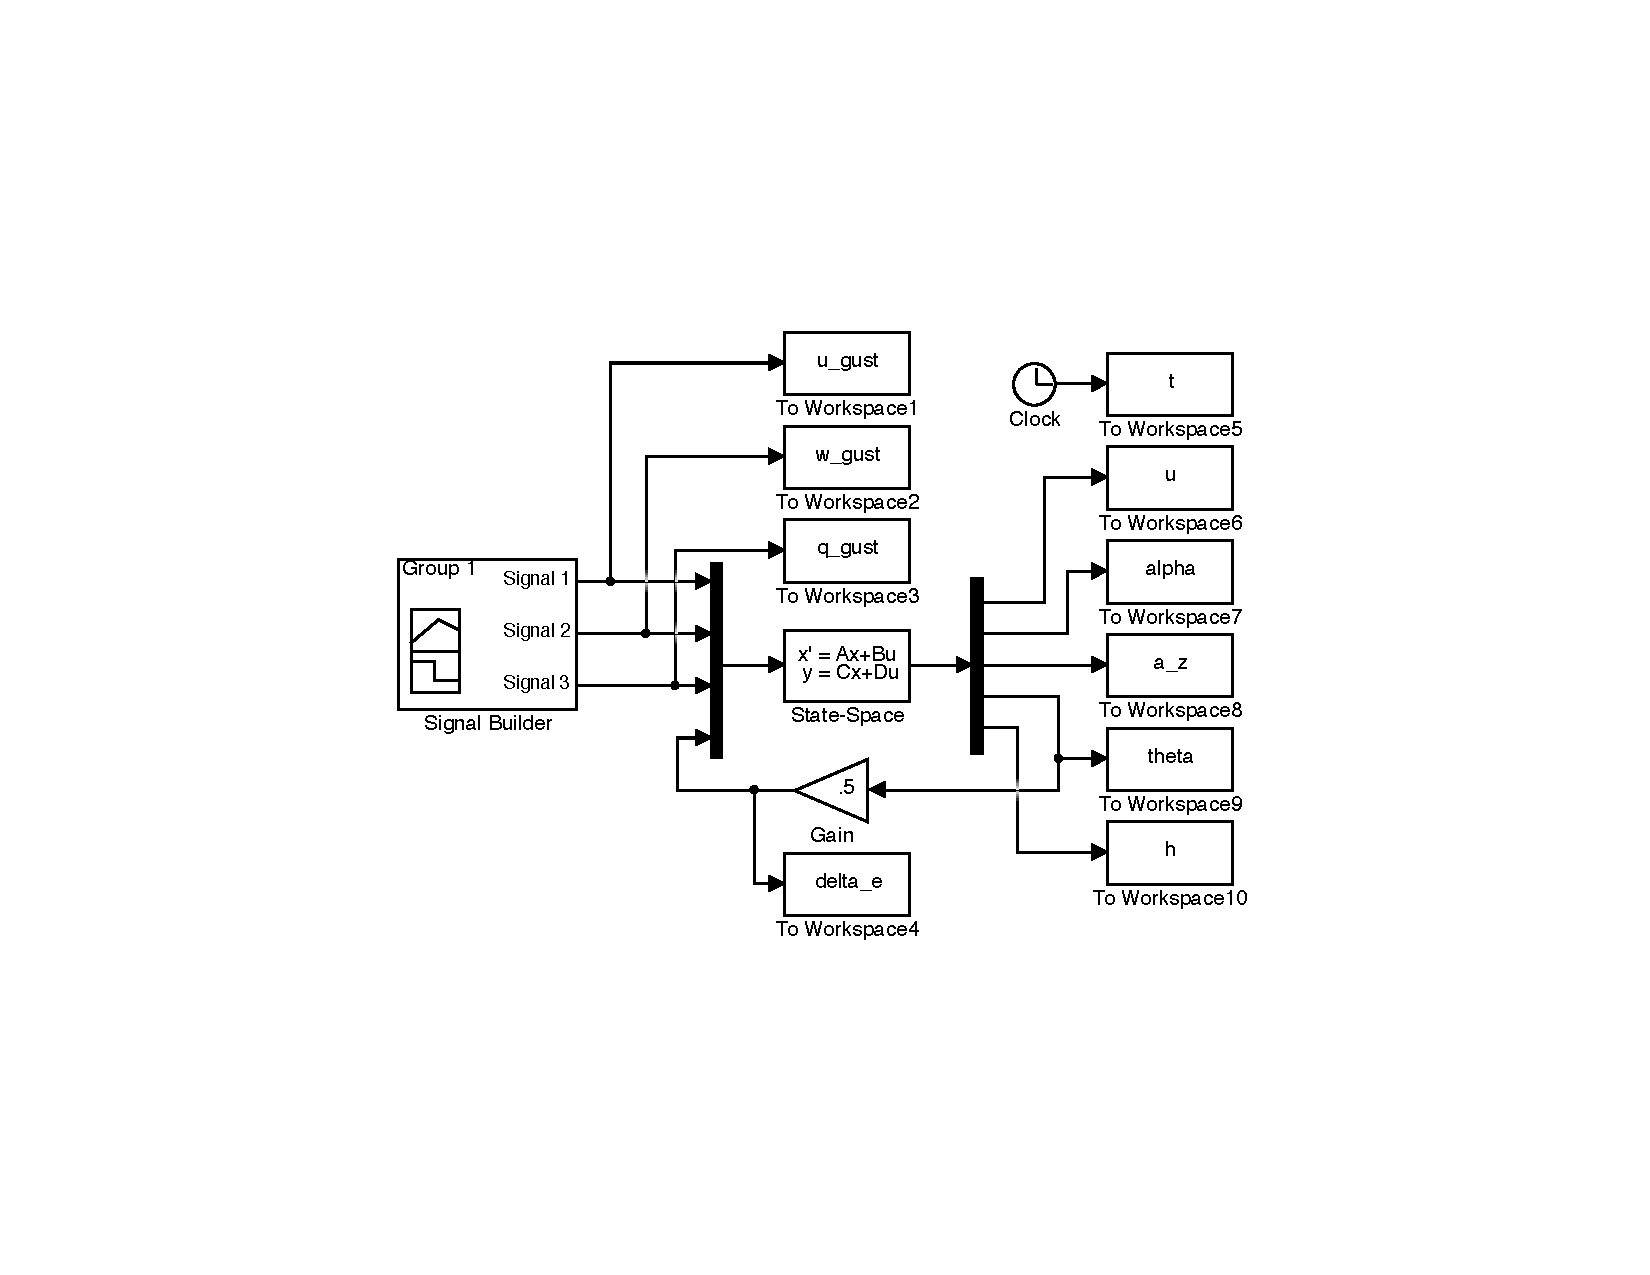
\includegraphics[width=.9\textwidth]{figures/simulink}
\caption{Simulink Diagram}
% \label{}
\end{center}
\end{figure}

\begin{figure}[h]
\begin{center}
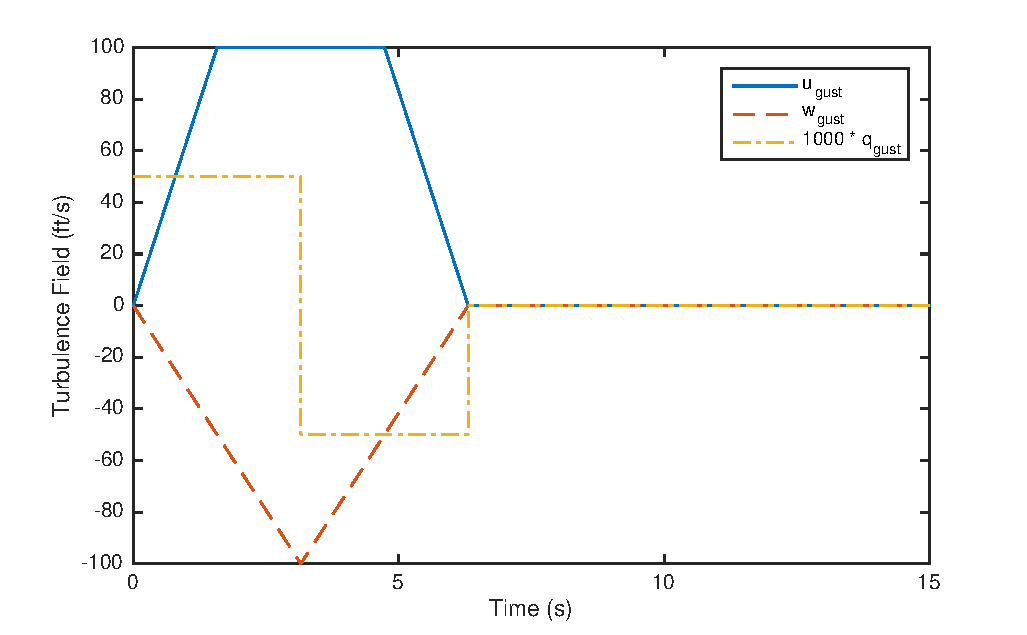
\includegraphics[width=.9\textwidth]{figures/gusts}
% \caption{Simulink Diagram}
% \label{}
\end{center}
\end{figure}

% \begin{figure}[h]
% \begin{center}
% 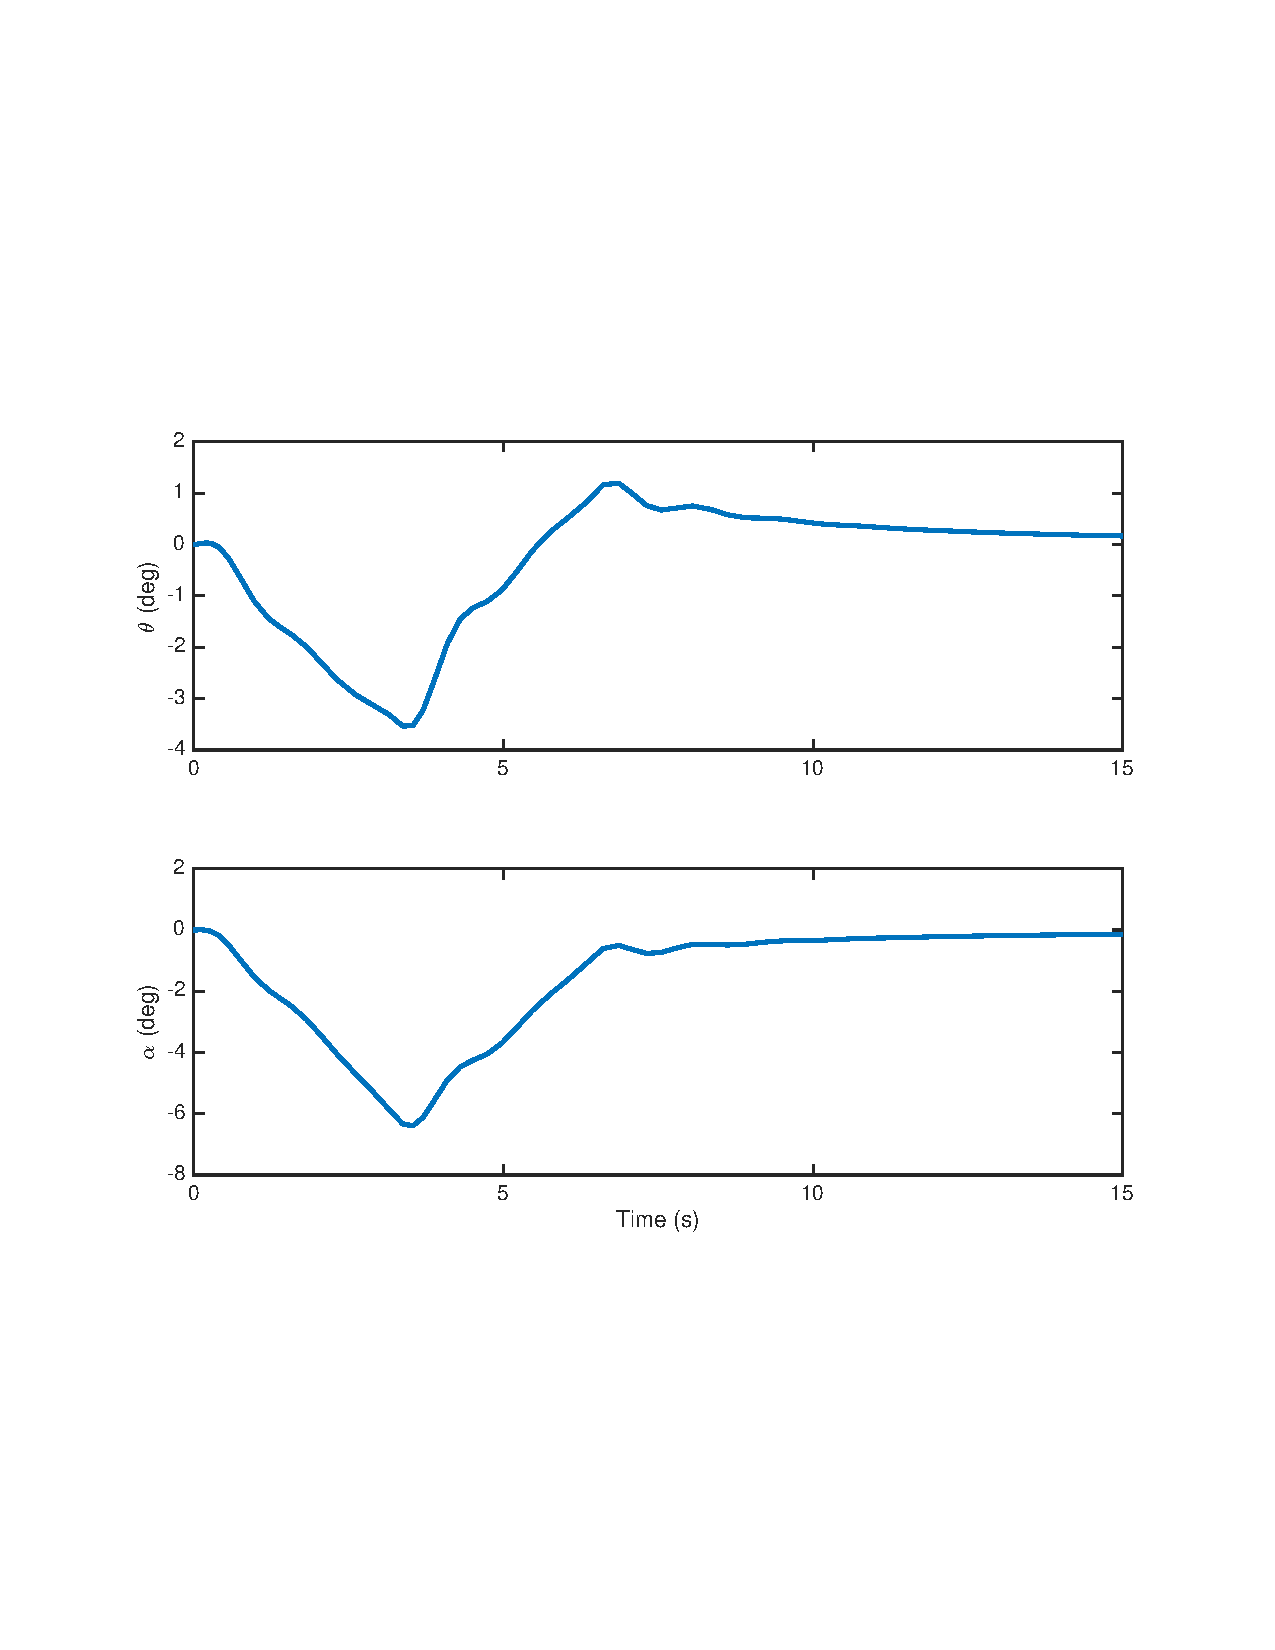
\includegraphics[width=1\textwidth]{figures/output angles}
% % \caption{Simulink Diagram}
% % \label{}
% \end{center}
% \end{figure}

% \begin{figure}[h]
% \begin{center}
% 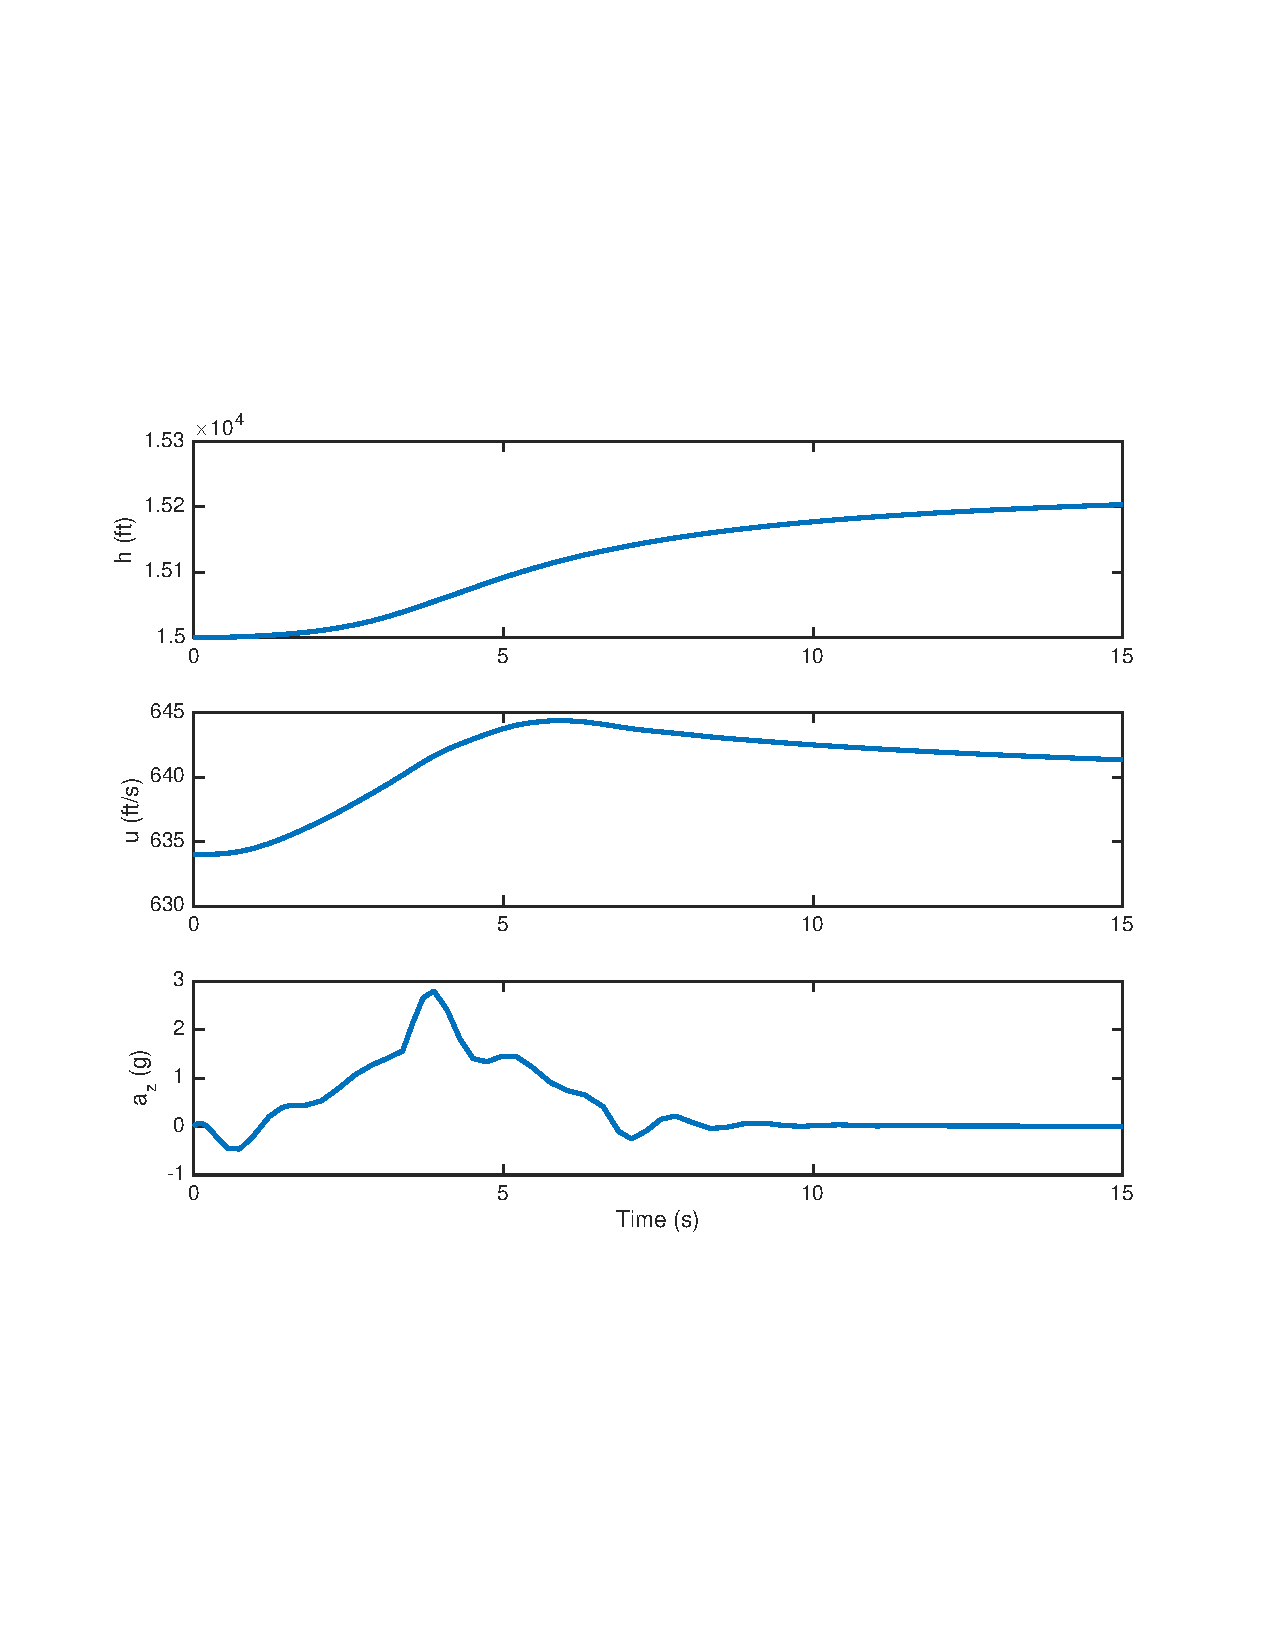
\includegraphics[width=1\textwidth]{figures/output x}
% % \caption{Simulink Diagram}
% % \label{}
% \end{center}
% \end{figure}

% \begin{figure}[h]
% \begin{center}
% 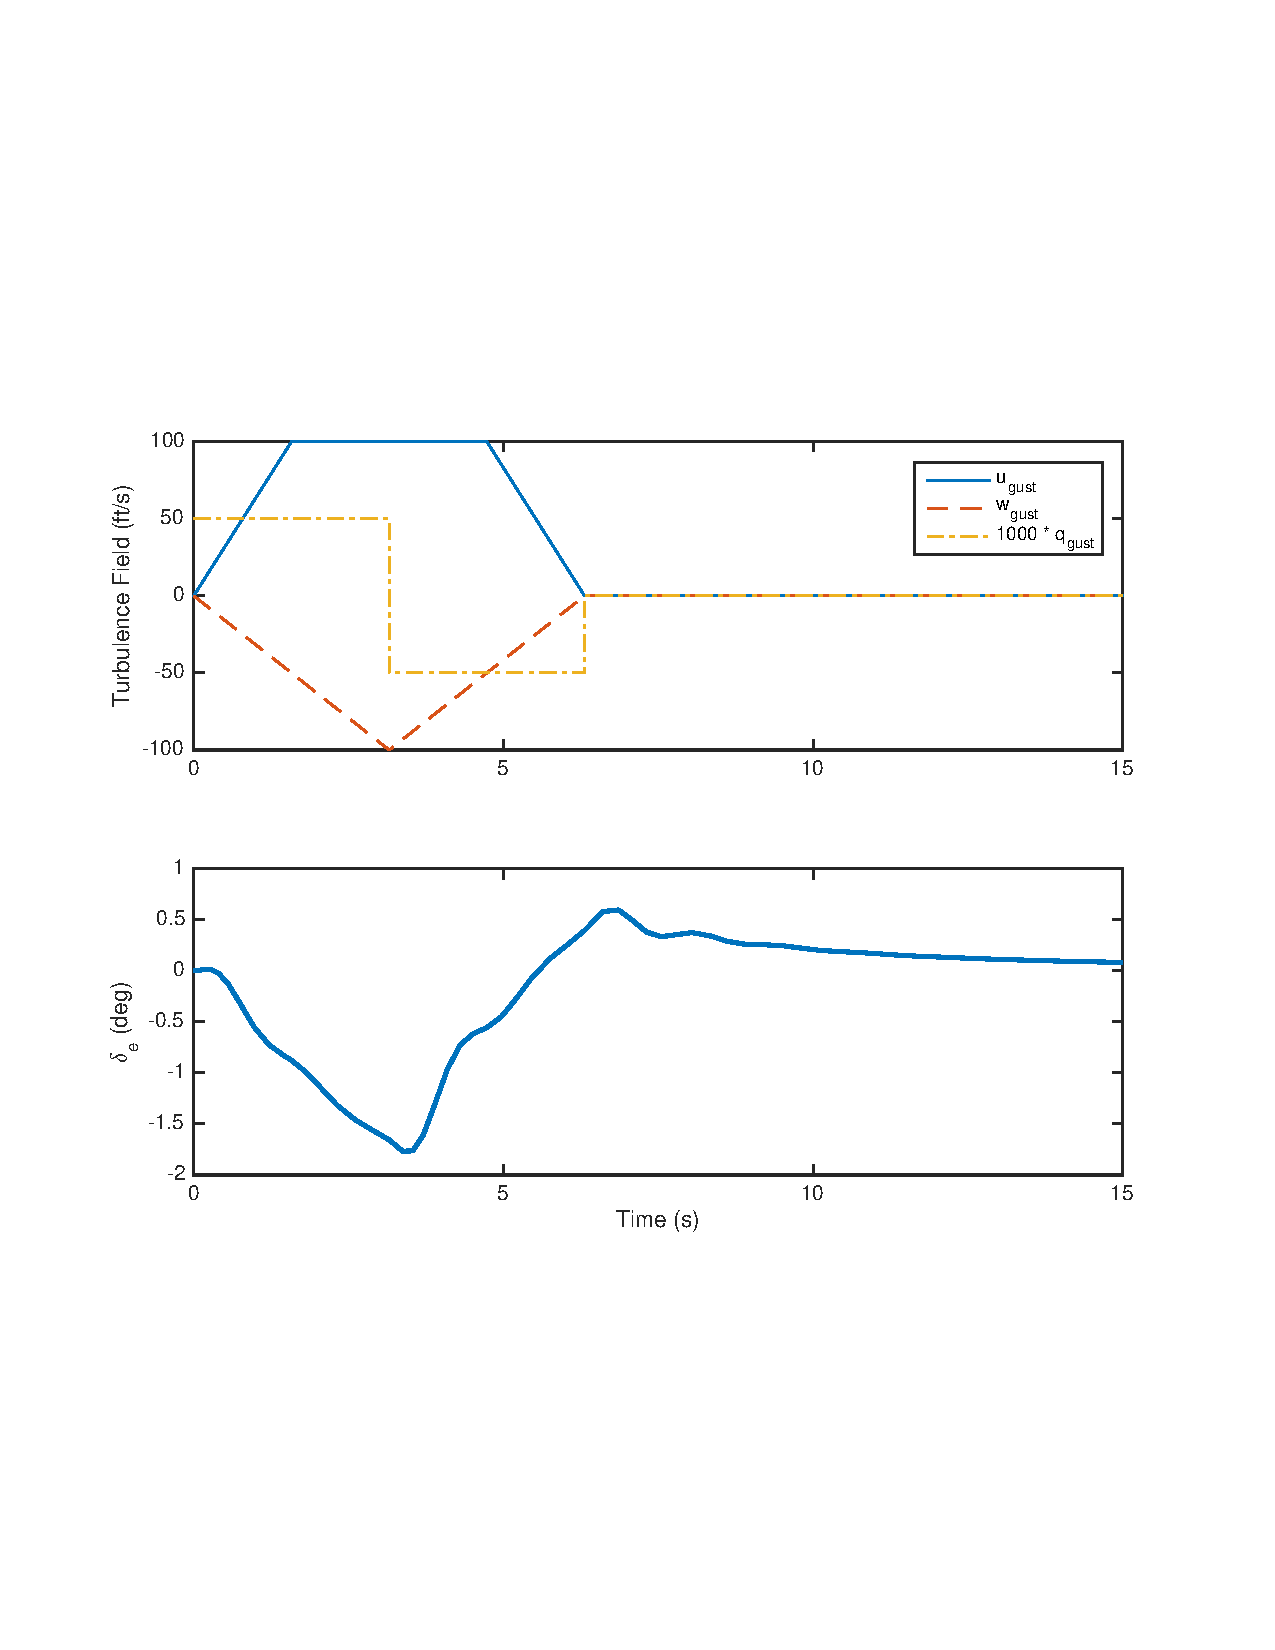
\includegraphics[width=1\textwidth]{figures/input}
% % \caption{Simulink Diagram}
% % \label{}
% \end{center}
% \end{figure}


\begin{figure}[h]
\begin{center}
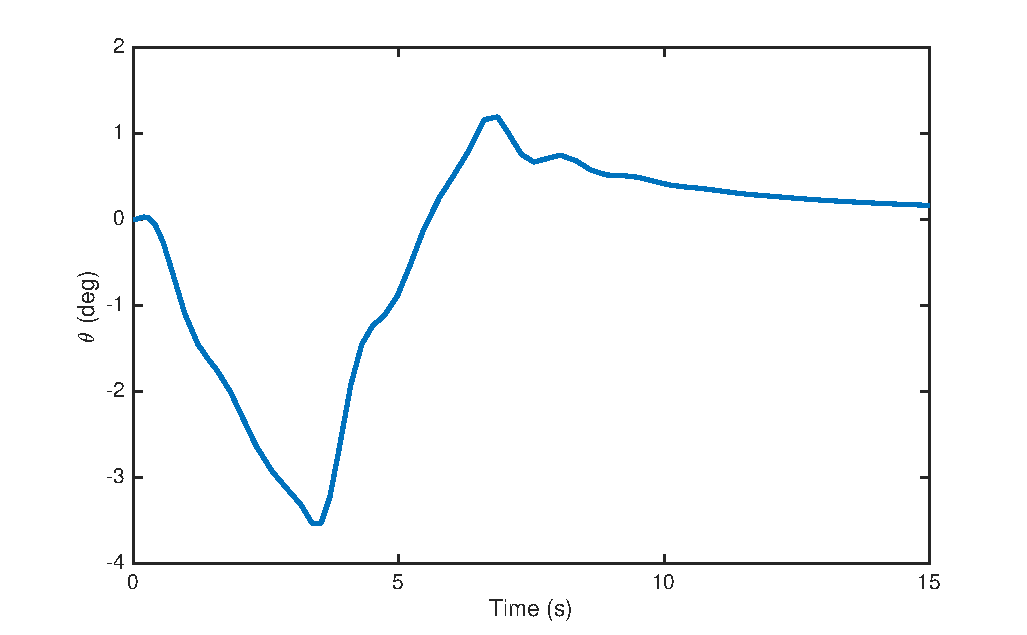
\includegraphics[width=1\textwidth]{figures/theta}
% \caption{Simulink Diagram}
% \label{}
\end{center}
\end{figure}
\begin{figure}[h]
\begin{center}
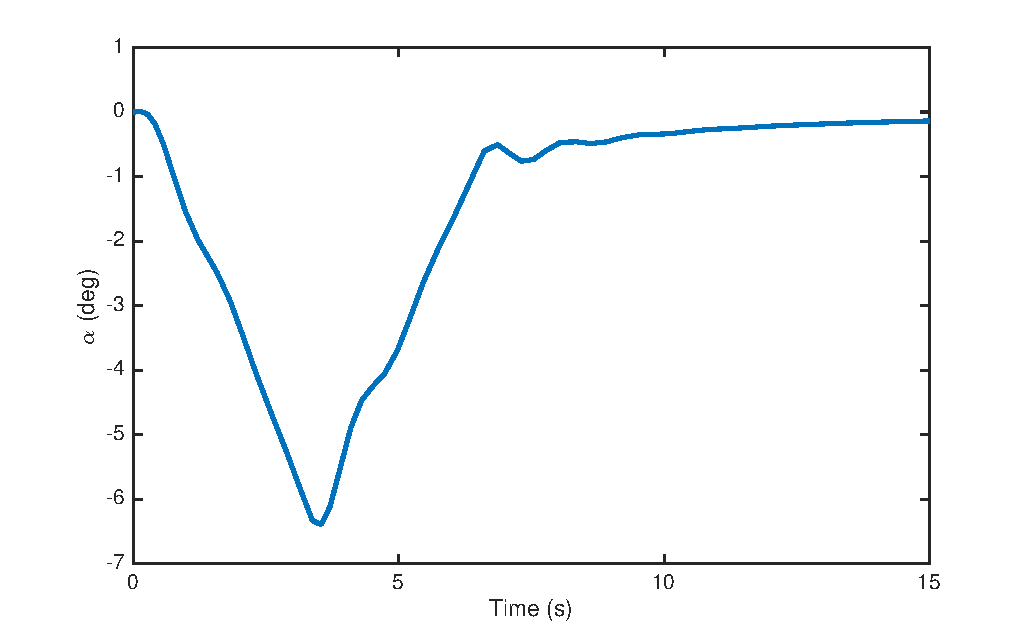
\includegraphics[width=1\textwidth]{figures/alpha}
% \caption{Simulink Diagram}
% \label{}
\end{center}
\end{figure}
\begin{figure}[h]
\begin{center}
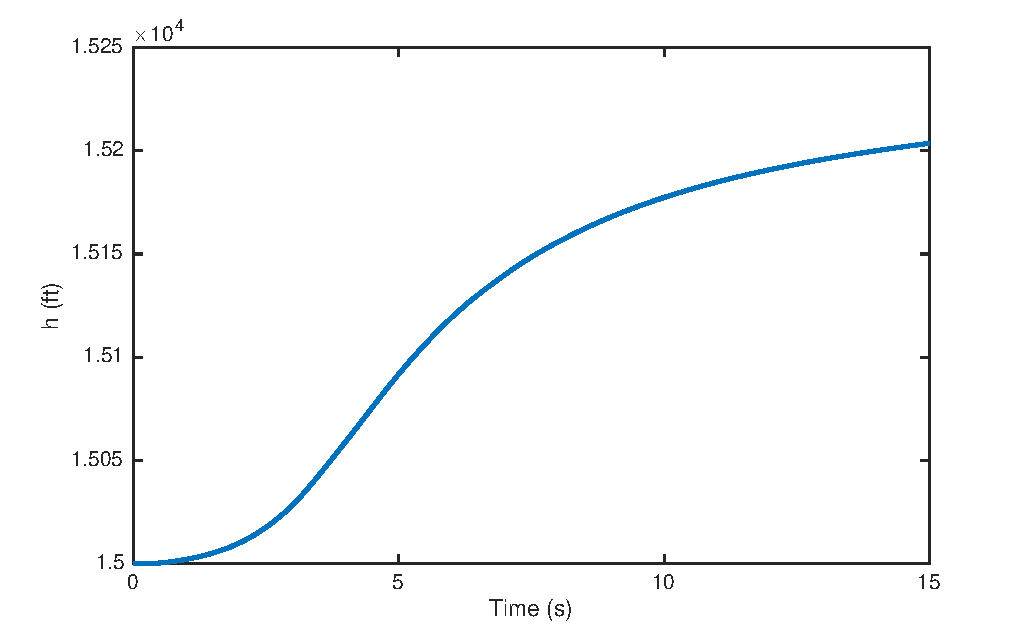
\includegraphics[width=1\textwidth]{figures/h}
% \caption{Simulink Diagram}
% \label{}
\end{center}
\end{figure}
\begin{figure}[h]
\begin{center}
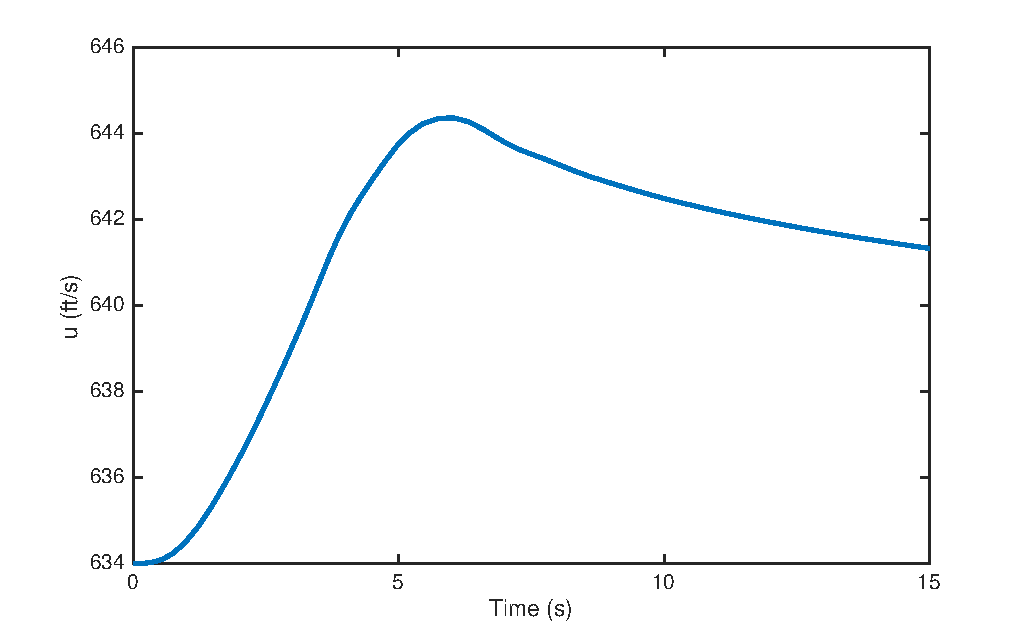
\includegraphics[width=1\textwidth]{figures/u}
% \caption{Simulink Diagram}
% \label{}
\end{center}
\end{figure}

\begin{figure}[h]
\begin{center}
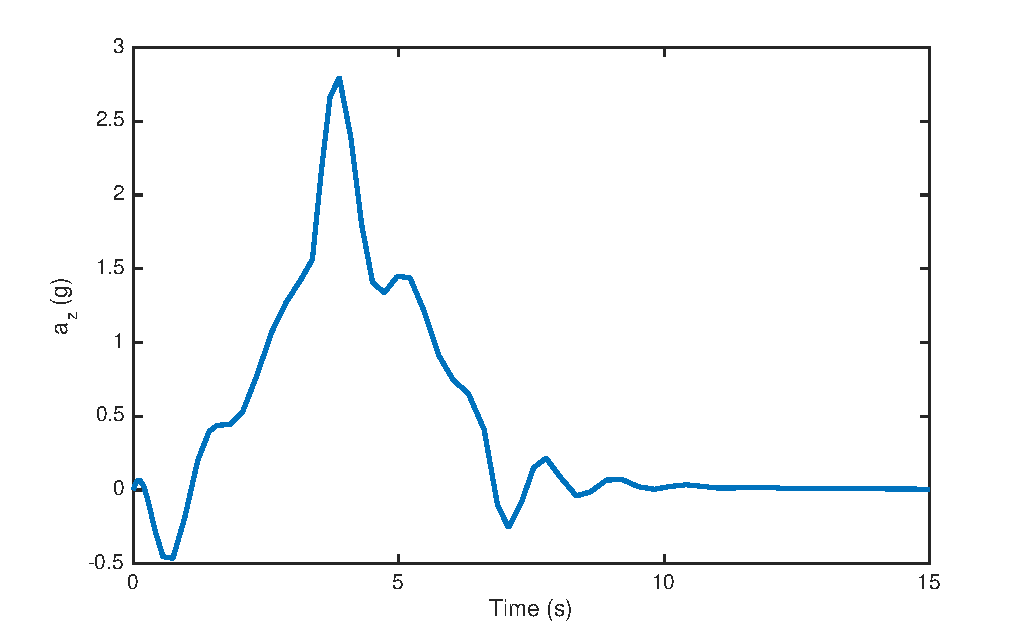
\includegraphics[width=1\textwidth]{figures/a_z}
% \caption{Simulink Diagram}
% \label{}
\end{center}
\end{figure}

\begin{figure}[h]
\begin{center}
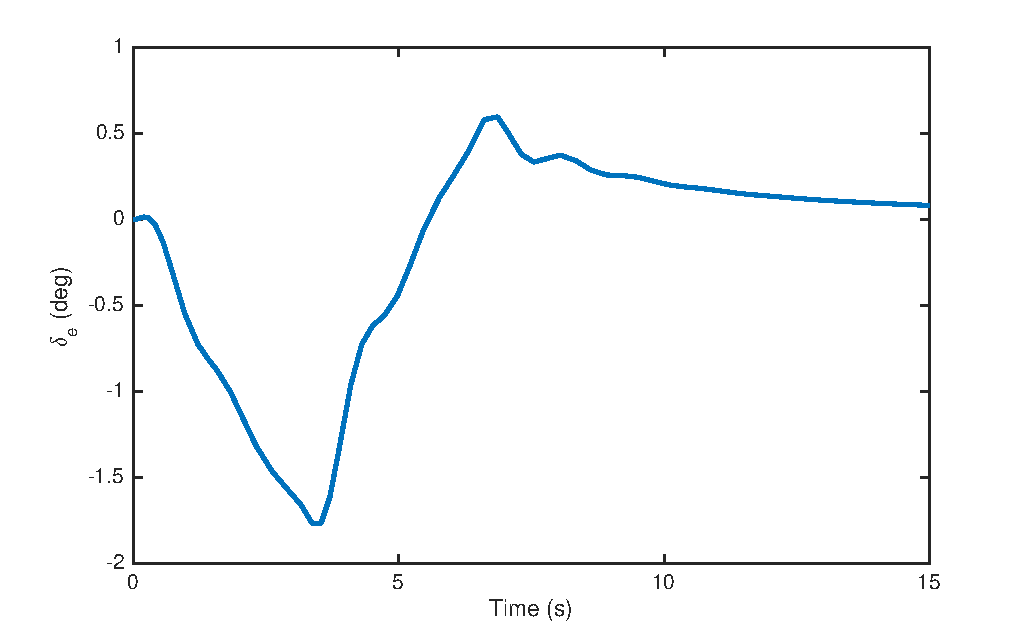
\includegraphics[width=1\textwidth]{figures/delta_e}
% \caption{Simulink Diagram}
% \label{}
\end{center}
\end{figure}

\end{document}
